\documentclass{article}

\usepackage{fouriernc,eulervm}
\usepackage[T1]{fontenc}
\usepackage[english]{babel}
\usepackage{float}
\usepackage{xcolor}
\usepackage[fleqn]{amsmath}

% Set page size and margins
% Replace `letterpaper' with`a4paper' for UK/EU standard size
\usepackage[a4paper,top=2cm,bottom=2cm,left=3cm,right=3cm,marginparwidth=1.75cm]{geometry}


% Useful packages
\usepackage{graphicx}
\usepackage[colorlinks=true, allcolors=blue]{hyperref}

\title{Random Forest for yield prediction on German NUTS3 Regions}

\author{Vincent Dlugosch}

\begin{document}

\date{August 14, 2024}

\maketitle
\begin{abstract}
	This experiment uses a random forest machine learning model to predict yearly yield anomalies for winter wheat in NUTS3 regions of Germany. The model is trained on climate data, derived climate indices, and static regional parameters. We explore two feature selection variants and evaluate the model's performance using data from 1979 to 2021.
\end{abstract}

\tableofcontents
\section{Introduction}
We use a random forest machine learning model to predict the yearly yield anomalies for winter wheat for NUTS3 regions in Germany. Training data consists of climate data, derived values from climate data such as SPI (Standard Precipitation Index), Days in the 99th percentile of wind speed per month, and monthly frost days among others. To account for regional differences we also include the average yield of each region in some of the model runs.
\section{Data Used}
As data for model training, we use 3 types of data. The data is averaged over each German NUTS3 region masked by the area where winter wheat was grown in the year 2018.
\subsection{Historical Climate Data}
This data, containing the climate variables: precipitation (pr), solar radiation (rsds), relative humidity (hurs), maximum temperature (tasmax), minimum temperature (tasmin), daily average temperature (tas), and wind speed (sfcWind) is available as daily data from 1979 to 2023 in 1 km * 1 km resolution over Germany.
It is resampled to monthly means and, as described before, subsequently averaged over each region masked by areas where winter wheat is grown. An example is show in \ref{fig:DE80J_cropped_example})

\begin{figure}[H]
	\centering
	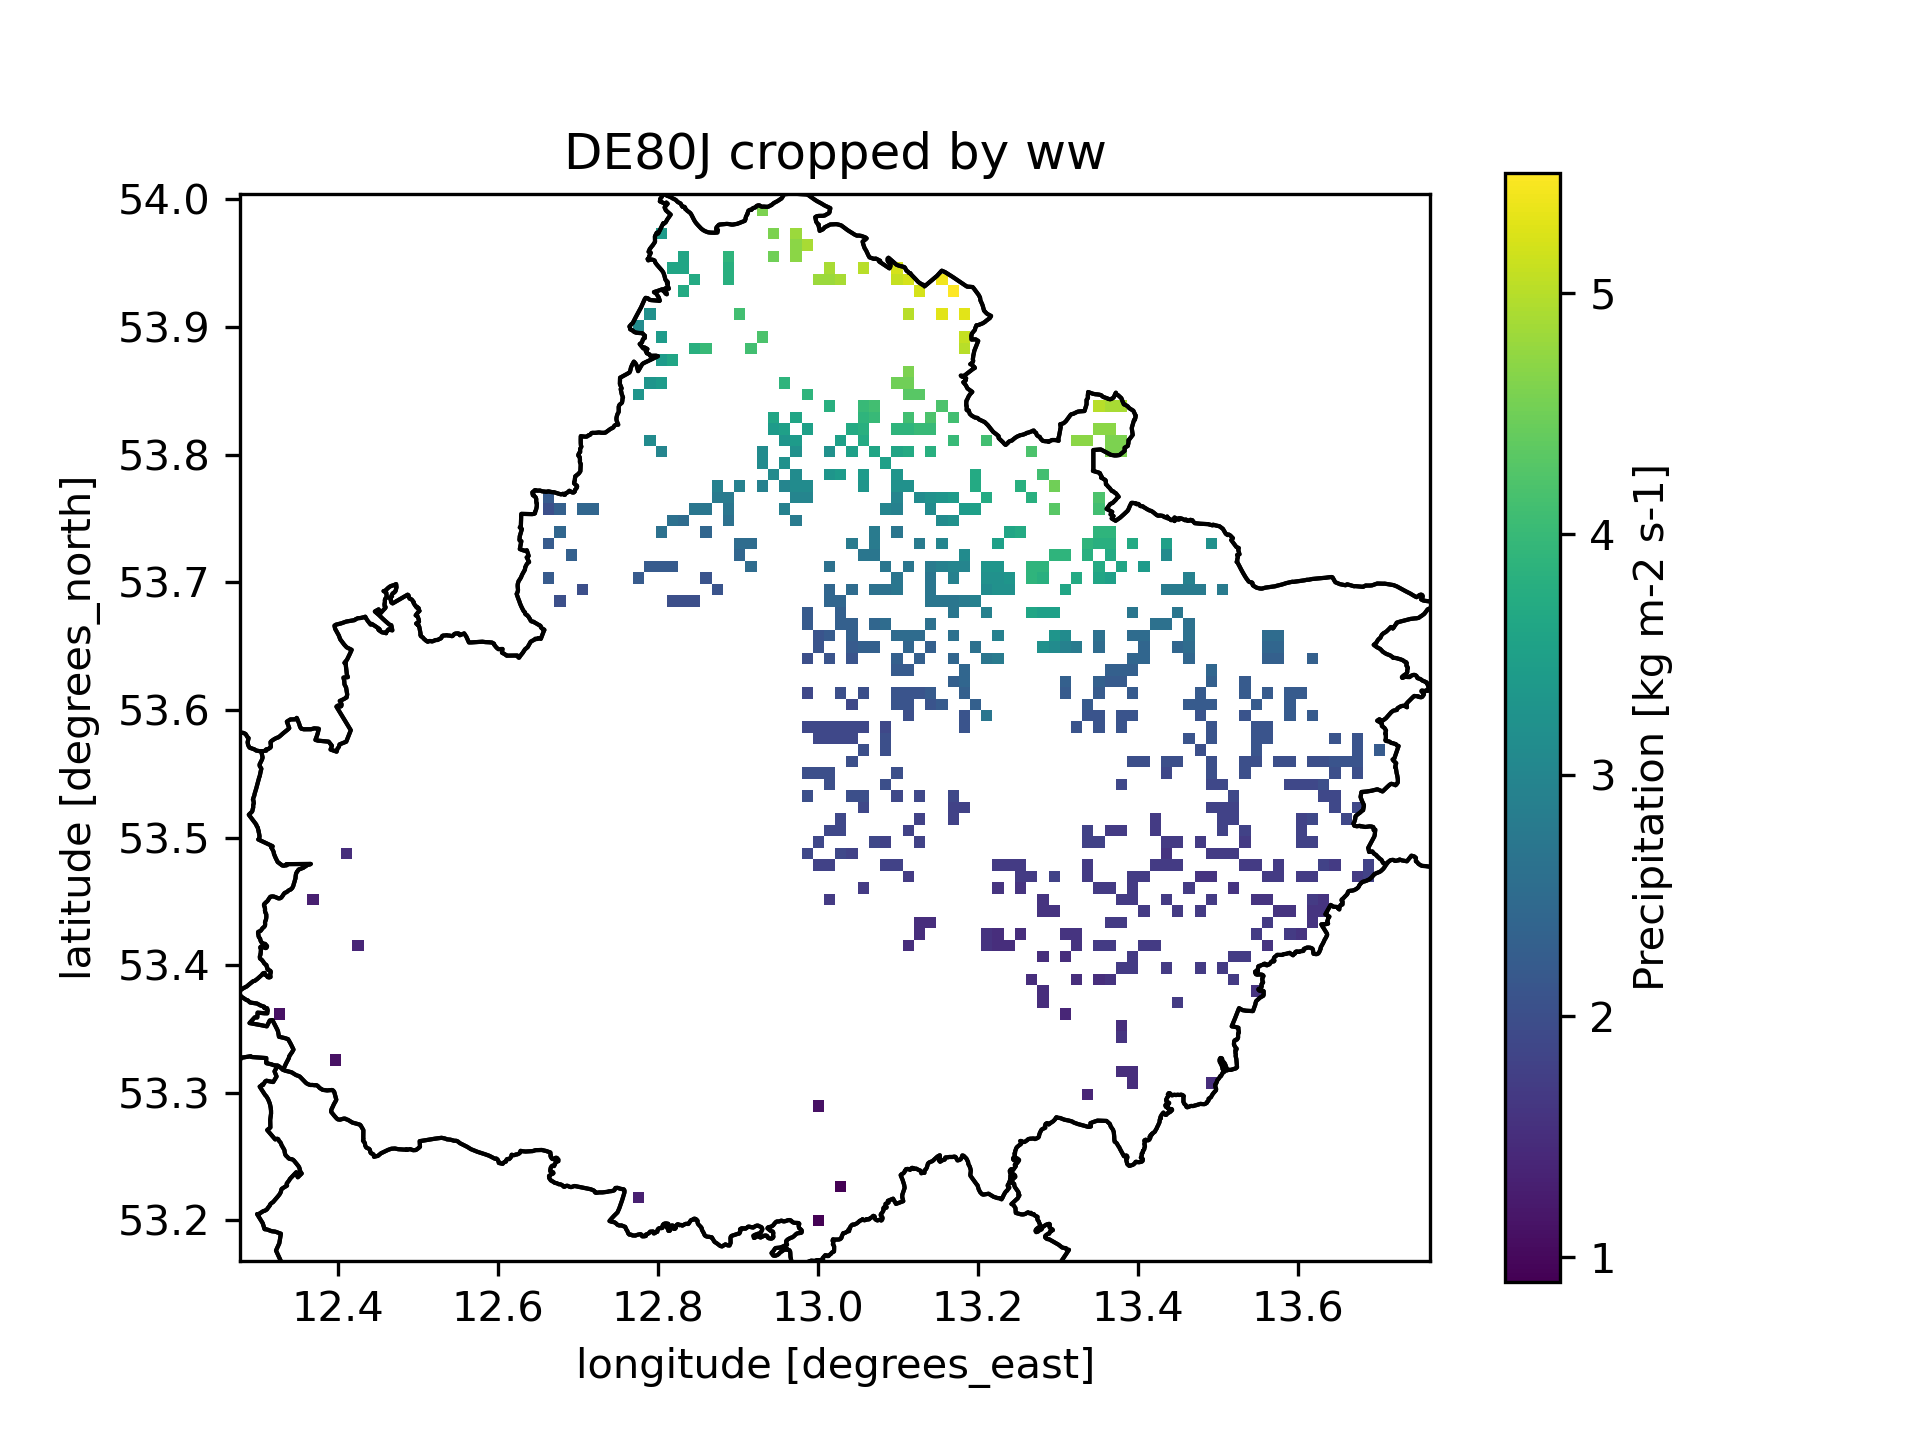
\includegraphics[width=0.8\textwidth]{./plots/DE80J_cropped_by_ww.png}
	\caption{\label{fig:DE80J_cropped_example}This graph shows how the climate data is broken down on a regional level all filled in dots show data used for aggregation. It is the specific region observed cropped by the winter wheat acreage.}
\end{figure}

\subsection{Derived Data}
This data is derived from the climate data. It includes:
\begin{itemize}
	\item SPI (Standard Precipitation Index) indicating periods of prolonged drought or abundance of precipitation compared to the observed time frame.
	\item Frost Days: Monthly sum of days when temperature is below 0 °C.
	\item Extreme wind days: days in the 99th percentile of extreme wind per month.
	\item Extreme precipitation days: days in the 99th percentile of precipitation per month.
	\item Heat Stress Days: The amount of days a certain threshold temperature is reached in a week. The threshold is 28 °C.
\end{itemize}
This data is also averaged over the regions and winter wheat acreage.
\subsection{Static Data}
This data is static data mapped to each NUTS3 region without any temporal resolution. We considered using elevation data, average temperature in the region over the observed period, and average precipitation for the region. In the end we just settled for the historic average yield for each region as it contains all the information necessary to capture regional differences. Sacrificing measurements of impact of other static data points in favor of model performance. It is also cropped by winter wheat acreage.
\subsection{Yield Data}
Yield data ranging from 1979 to 2021 is available. Tons per acre data is available for 397 NUTS3 regions in Germany for various crops. As the model is only optimized for winter wheat, yield data for that crop is extracted. The yield data is processed to obtain weighted percentage values of yield anomalies compared to the 5-year period previous to the most recent year for the observed year. We observe a subset of regions where at least 15 squares of winter wheat are grown and where at least 40 of the 43 years of data are available. This leads to 242 of the 397 regions used.
\section{Features}
Five different subsets of features are used to observe the impact of different feature arrangement. This provides a good starting point for further feature selection or exclusion.
\subsection{Features used}
Following is a list of features used when looking at all variants. Each variant uses a subset of this list:
\begin{itemize}
	\item Mean regional yield for per region
	\item Monthly SPI values per region and year
	\item Monthly frost days per region and year
	\item Monthly days of extreme wind per region and year
	\item Monthly days of extreme precipitation per region and year
	\item Weekly heat stress days per region and year
	\item Monthly precipitation values per region and year
	\item Monthly solar radiation values per region and year
	\item Monthly average temperature values per region and year
	\item Monthly minimum temperature values per region and year
	\item Monthly maximum temperature values per region and year
	\item Monthly relative humidity values per region and year
	\item Monthly wind speed values per region and year
\end{itemize}
\subsection{Feature variants}
\subsubsection{Variant 1}
In this variant only mean regional yield is used to predict future yields.
\subsubsection{Variant 2}
In this variant the derived features like frost days and SPI are used in conjunction with the mean regional yield.
\subsubsection{Variant 3}
In this variant the derived features like frost days and SPI are used without the mean regional yield.
\subsubsection{Variant 4}
In this variant monthly raw data is used in conjunction with the mean regional yield.
\subsubsection{Variant 5}
In this variant monthly raw data is used without the mean regional yield.
\section{Methods}
\subsection{Random Forest}
The model is built using the ''scikit-learn`` python library's ''RandomForestRegressor``.
\subsubsection{Node feature relationship}
Each node corresponds to one feature when building the tree. The algorithm takes a subset of features on each node and tries to find the best feature and corresponding threshold to make the split on. Different thresholds are tried. For classification problems such as binary classification problems, the goal is to maximize the information gain for each split.
For regression problems, the variance of the target variable is tried to be minimized by trying different combinations of features and thresholds. The lower the variance, the better the quality of the split.
\subsubsection{Bootstrapping}
Each decision tree in the random forest is constructed using a bootstrapped dataset. Meaning a new dataset is created of the same size as the original with the difference that samples from the original dataset can be either omitted or appear multiple times in the bootstrapped dataset.
\subsubsection{Aggregation}
The random forest makes a prediction on the input data using each tree in the forest. The result is then aggregated using the average of all results.
The combination of "Bootstrapping" and "Aggregation" is called Bagging.
\subsubsection{Split calculation}
\begin{alignat*}{2}
	 & Weighted MSE &  & = w_L \cdot MSE_L + w_R \cdot MSE_R                \\
	 & where:       &  &                                                    \\
	 & w_L          &  & = \frac{n_L}{n_{total}}                            \\
	 & w_R          &  & = \frac{n_R}{n_{total}}                            \\
	 & MSE_L        &  & = \frac{1}{n_L} \sum_{i \in L} (y_i - \bar{y}_L)^2 \\
	 & MSE_R        &  & = \frac{1}{n_R} \sum_{i \in R} (y_i - \bar{y}_R)^2 \\
	 & \bar{y}_L    &  & = \frac{1}{n_L} \sum_{i \in L} y_i                 \\
	 & \bar{y}_R    &  & = \frac{1}{n_R} \sum_{i \in R} y_i                 \\
	 & n_L          &  & = \text{Number of samples in the left split}       \\
	 & n_R          &  & = \text{Number of samples in the right split}      \\
	 & n_{total}    &  & = n_L + n_R
\end{alignat*}


\subsubsection{Example}
\textbf{Split decision on node one:}
\\
\textbf{Split between SPI -2 and -1}

$n_L = 1, \ n_R = 4, \ n_{total} = 5, \ w_L = \frac{1}{5} = 0.2, \ w_R = \frac{4}{5} = 0.8$

$\bar{y}_L = -2$

$\bar{y}_R = \frac{(-1 + 1 + 1.2 + 1.7)}{4} = 0.725$

$MSE_L = (-5 + 2)^2 = 9$

$MSE_R = (-1 - 0.725)^2 + (1 - 0.725)^2 + (10 - 0.725)^2 + (12 - 0.725)^2 = 3 + 0.075 + 86 + 127 = 216.1$

$Weighted MSE = w_L \cdot MSE_L + w_R \cdot MSE_R = 0.2 \cdot 9 + 0.8 \cdot 216.1 = 174.6$
\\
\textbf{Split between SPI -1 and 1}

$n_L = 2, \ n_R = 3, \ n_{total} = 5, \ w_L = \frac{2}{5} = 0.4, \ w_R = \frac{3}{5} = 0.6$

$\bar{y}_L = \frac{(-2 - 1)}{2} = -1.5$

$\bar{y}_R = \frac{(1 + 1.2 + 1.7)}{3} = 1.3$

$MSE_L = (-5 + 1.5)^2 + (2 + 1.5)^2 = 12.25 + 12.25 = 25$

$MSE_R = (3 - 1.3)^2 + (10 - 1.3)^2 + (12 - 1.3)^2 = 2.89 + 75.69 + 114.49 = 193.07$

$Weighted MSE = w_L \cdot MSE_L + w_R \cdot MSE_R = 0.4 \cdot 25 + 0.6 \cdot 193.07 = 125.842$
\\
\textbf{Split between SPI 1 and 1.2}

$n_L = 3, \ n_R = 2, \ n_{total} = 5, \ w_L = \frac{3}{5} = 0.6, \ w_R = \frac{2}{5} = 0.4$

$\bar{y}_L = \frac{(-2 - 1 + 1)}{3} = -1$

$\bar{y}_R = \frac{(1.2 + 1.7)}{2} = 1.45$

$MSE_L = (-5 + 1)^2 + (2 + 1)^2 + (3 + 1)^2 = 16 + 9 + 16 = 41$

$MSE_R = (10 - 1.45)^2 + (12 - 1.45)^2 = 73.1 + 111.3 = 184.4$

$Weighted MSE = w_L \cdot MSE_L + w_R \cdot MSE_R = 0.6 \cdot 41 + 0.4 \cdot 184.4 =$\colorbox{yellow}{$98.36$}
\\
\textbf{Split between SPI 1.2 and 1.7}

$n_L = 4, \ n_R = 1, \ n_{total} = 5, \ w_L = \frac{4}{5} = 0.8, \ w_R = \frac{1}{5} = 0.2$

$\bar{y}_L = \frac{(-1 - 2 + 1 + 1.2)}{4} = -0.2$

$\bar{y}_R = 1.7$

$MSE_L = (-5 + 0.2)^2 + (2 + 0.2)^2 + (3 + 0.2)^2 + (10 + 0.2)^2 = 23.04 + 4.84 + 10.24 + 104.04 = 142.16$

$MSE_R = (12 - 1.7)^2 = 106.09$

$Weighted MSE = w_L \cdot MSE_L + w_R \cdot MSE_R = 0.8 \cdot 142.16 + 0.2 \cdot 106.09 = 135.34$
\\
\textbf{Split decision on node two:}
\\
\textbf{Split between SPI -2 and -1}

$n_L = 1, \ n_R = 2, \ n_{total} = 3, \ w_L = \frac{1}{3} = 0.33, \ w_R = \frac{2}{3} = 0.66$

$\bar{y}_L = -2$

$\bar{y}_R = 0$

$MSE_L = (-5 + 2)^2 = 9$

$MSE_R = 2^2 + 3^2 = 4 + 9 = 13$

$Weighted MSE = w_L \cdot MSE_L + w_R \cdot MSE_R = 0.33 \cdot 9 + 0.66 \cdot 13 =$\colorbox{yellow}{$11.58$}
\noindent
\\
\textbf{Split between SPI -1 and 1 }

$n_L = 2, \ n_R = 1, \ n_{total} = 3, \ w_L = \frac{2}{3} = 0.66, \ w_R = \frac{1}{3} = 0.33$

$\bar{y}_L = -1.5$

$\bar{y}_R = 1$

$MSE_L = (-5 + 1.5)^2 + (2 + 1.5)^2 = 12.25 + 12.25 = 25$

$MSE_R = (3 - 1)^2 = 4$

$Weighted MSE = w_L \cdot MSE_L + w_R \cdot MSE_R = 0.66 \cdot 25 + 0.33 \cdot 4 = 17.99$

\begin{figure}[H]
	\centering
	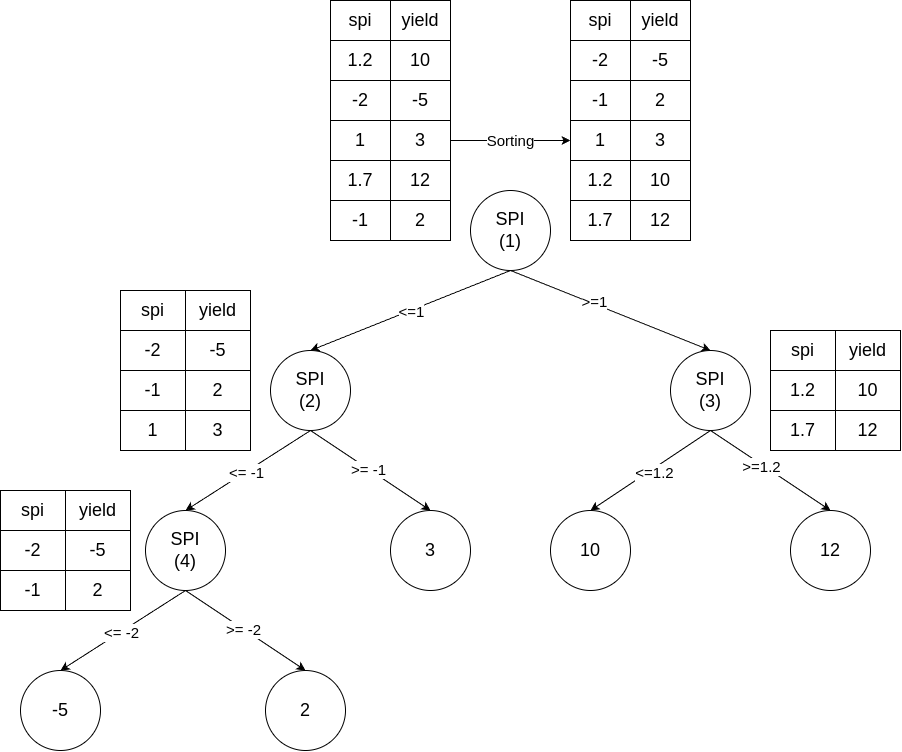
\includegraphics[width=1.0\textwidth]{./plots/DecisionTreeSplit.png}
	\caption{\label{fig:decision_tree_split}This Diagram illustrates how split decisions are taken in a decision tree.}
\end{figure}
\noindent
\subsubsection{Tree Parameters}
The random forest for all variants has a number of trees of from 100 to 500 the rest of the parameters are left at default. The number of trees is chosen by a time series based grid search.  A random state of 42 is used across the project to make the results reproducible.
The number of trees is chosen as the model performance does not degrade when adding more trees and no significant performance gains are observed after around 100 trees (Figure \ref{fig:n_trees_vs_performance}). Choosing  up to 500 trees gives headroom where the number of trees is not a performance constraint while still maintaining an acceptable speed of calculation for each random forest.
A max features value of 0.66 was used to increase diversity among trees. This parameter controlls the selection of features per tree built.

Further hyperparameter optimization is outstanding.
\begin{figure}[H]
	\centering
	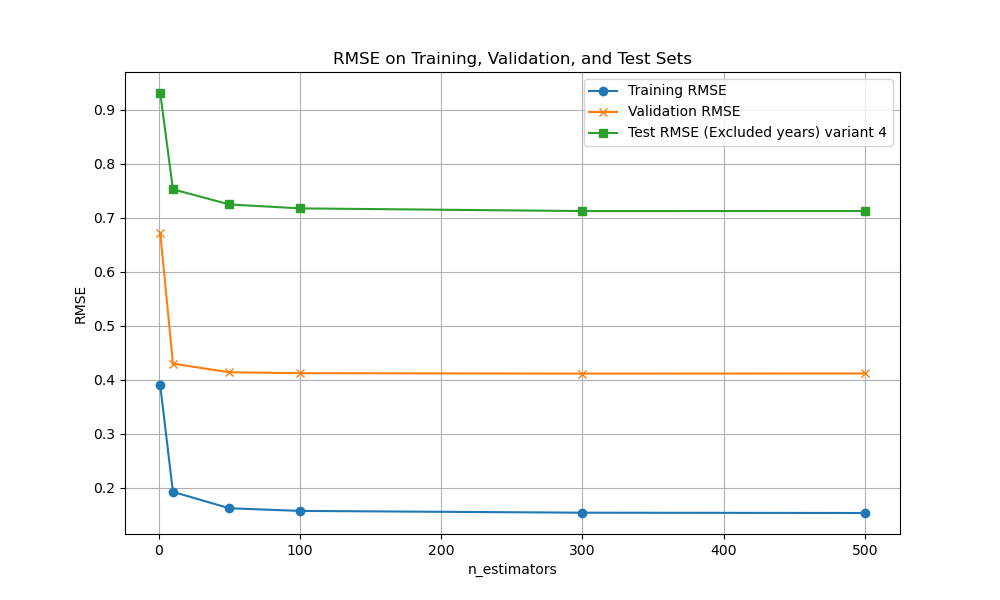
\includegraphics[width=1.0\textwidth]{./plots/n_trees_vs_error_variant_4.png}
	\caption{\label{fig:n_trees_vs_performance}This graph shows model performance based on the number of trees used (variant 4). No meaningful gains after about 100 trees.}
\end{figure}

\subsection{Data Handling}
For training and evaluating the model's performance, different sets of data are used.
\subsubsection{Training Data}
Training data is the data the model uses to construct its trees. It contains both the features and corresponding targets.
For this model, training data comprises a random selection of 90\% of the available data ranging from 1979 to 2021, excluding the years 2015 through 2021.
\subsubsection{Validation Data}
Validation data is used to assess the model's performance during hyperparameter optimization.
In this case, a random selection of 10\% of the available data ranging from 1979 to 2021, excluding the years 2015 through 2021, is used.
As we are dealing with time series data, a random selection to validate on brings the risk of contaminating the training data with information of the current year, and the model might perform better on this subset than on real data.
\subsubsection{Test Data}
To mitigate that risk, whole yearly time series are excluded from both the training and validation data. Namely, the years 2015 through 2021. This selection is more or less arbitrary.
The model is applied to the test data in the end to assess the model's real-world performance.
\section{Results}
All model variations perform well on the validation data. Except for variant one which is probably due to the limited number of features and univariate regression.
\subsection{Variant 1}
This variant only has the mean regional yield as feature to isolate that hugely important feature.
\subsubsection{Performance}
We can observe that the model predicts fairly well on the validation data with an R2 value of 0.69 both on training and validation data and still predicting fairly well on the excluded years with an R2 value of 0.47.
As can be seen in table \ref{table:errors_on_datasets_variant_1} and \ref{table:errors_on_datasets_years_variant_1}.
\begin{table}[H]
	\centering
	\begin{tabular}{lcccc}
		\hline
		Data Split                 & MSE  & RMSE & MAE  & R$^2$ \\
		\hline
		Training Data              & 0.29 & 0.54 & 0.43 & 0.69  \\
		Validation Data            & 0.30 & 0.55 & 0.43 & 0.69  \\
		Test (Excluded: 2015-2021) & 0.55 & 0.74 & 0.58 & 0.47  \\
		\hline
	\end{tabular}
	\caption{\label{table:errors_on_datasets_variant_1} Random Forest performance metrics for training, validation, and test sets. The test set excludes data from years 2015 to 2021 (variant 1).}
\end{table}

\begin{table}[H]
	\centering
	\begin{tabular}{lcccc}
		\hline
		Excluded Year & MSE  & RMSE & MAE  & R$^2$ \\
		\hline
		2015          & 0.38 & 0.61 & 0.47 & 0.63  \\
		2016          & 0.62 & 0.78 & 0.63 & 0.31  \\
		2017          & 0.41 & 0.64 & 0.50 & 0.53  \\
		2018          & 0.91 & 0.95 & 0.78 & 0.35  \\
		2019          & 0.54 & 0.74 & 0.57 & 0.59  \\
		2020          & 0.64 & 0.80 & 0.66 & 0.40  \\
		2021          & 0.36 & 0.60 & 0.48 & 0.52  \\
		\hline
	\end{tabular}
	\caption{\label{table:errors_on_datasets_years_variant_1} Random Forest performance metrics for test sets with individual years excluded.}
\end{table}

\begin{figure}[H]
	\centering
	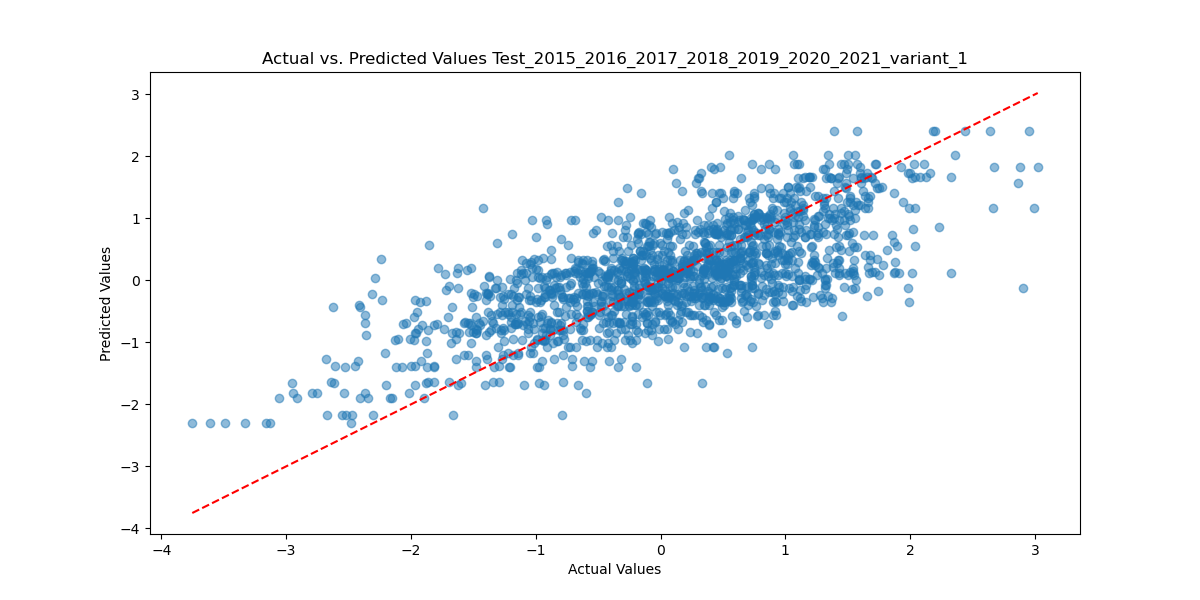
\includegraphics[width=1.0\textwidth]{./plots/scatter_Test_2015_2016_2017_2018_2019_2020_2021_variant_1.png}
	\caption{\label{fig:scatter_excluded_years_variant_1}This scatter plot shows the relationship between prediction and real values of excluded years (variant 1).}
\end{figure}

\subsubsection{Feature importance}
We get feature importance values for each Feature here the only and most important features are shown (Table \ref{table:feature_importance_variant_1}).
As only one feature was included we have feature importance of 100 percent.
\begin{table}[H]
	\centering
	\begin{tabular}{lc}
		\hline
		Feature                   & Importance \\
		\hline
		mean\_regional\_ww\_yield & 1.000000   \\
		\hline
	\end{tabular}
	\caption{\label{table:feature_importance_variant_1} Feature importance for variant one.}
\end{table}


\subsection{Variant 2}
This variant combines derived features and the mean regional yield for prediction.
\subsubsection{Performance}
The model performs well on the training and validation sets with an R2 of 0.97 and 0.80 respectively fitting strongly to training data and performing way better on validation data. However, it generalizes worse on excluded years like all models but increases its accuracy a little bit compared to variant 1, achieving an R2 of 0.49 when all excluded years are considered. The model's performance on individual excluded years varies, with some years showing better performance than others. For instance, the R2 score for 2015 is 0.60, while the R2 for 2018 is only 0.36.
As can be seen in table \ref{table:errors_on_datasets_variant_2} and \ref{table:errors_on_datasets_years_variant_2}.
\begin{table}[H]
	\centering
	\begin{tabular}{lcccc}
		\hline
		Data Split                 & MSE  & RMSE & MAE  & R$^2$ \\
		\hline
		Training Data              & 0.03 & 0.17 & 0.13 & 0.97  \\
		Validation Data            & 0.19 & 0.44 & 0.33 & 0.80  \\
		Test (Excluded: 2015-2021) & 0.53 & 0.73 & 0.57 & 0.49  \\
		\hline
	\end{tabular}
	\caption{\label{table:errors_on_datasets_variant_2} Random Forest performance metrics for training, validation, and test sets. The test set excludes data from years 2015 to 2021 (variant 2).}
\end{table}

\begin{table}[H]
	\centering
	\begin{tabular}{lcccc}
		\hline
		Excluded Year & MSE  & RMSE & MAE  & R$^2$ \\
		\hline
		2015          & 0.40 & 0.63 & 0.48 & 0.60  \\
		2016          & 0.53 & 0.73 & 0.58 & 0.40  \\
		2017          & 0.41 & 0.64 & 0.50 & 0.53  \\
		2018          & 0.89 & 0.94 & 0.76 & 0.36  \\
		2019          & 0.54 & 0.73 & 0.57 & 0.59  \\
		2020          & 0.61 & 0.78 & 0.63 & 0.42  \\
		2021          & 0.36 & 0.60 & 0.48 & 0.53  \\
		\hline
	\end{tabular}
	\caption{\label{table:errors_on_datasets_years_variant_2} Random Forest performance metrics for test sets with individual years excluded.}
\end{table}

\begin{figure}[H]
	\centering
	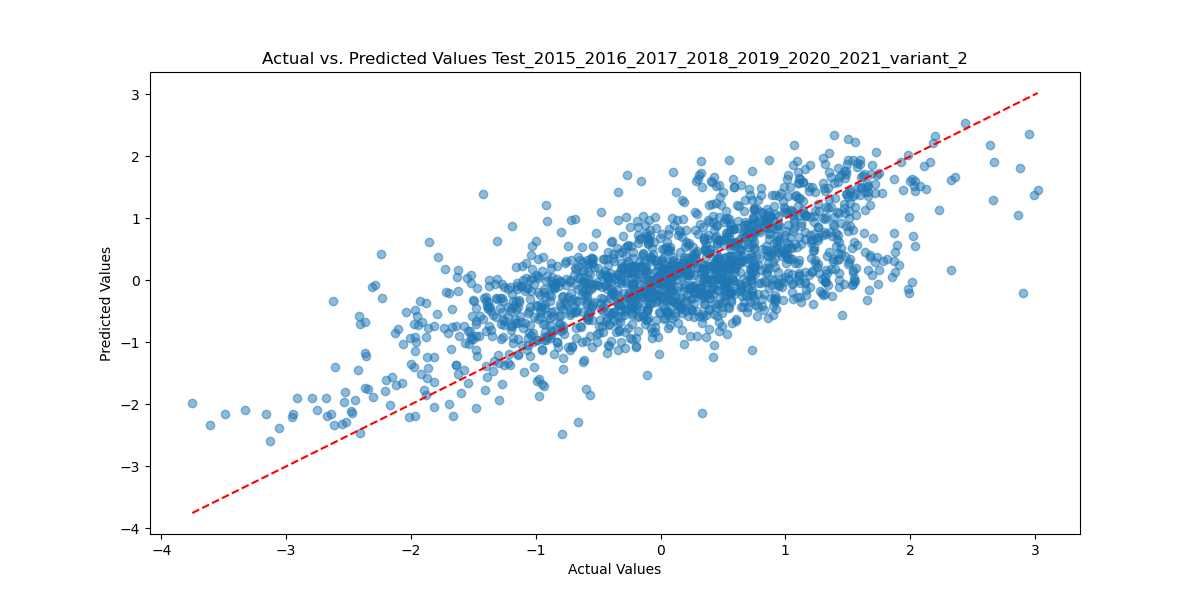
\includegraphics[width=1.0\textwidth]{./plots/scatter_Test_2015_2016_2017_2018_2019_2020_2021_variant_2.png}
	\caption{\label{fig:scatter_excluded_years_variant_2}This scatter plot shows the relationship between prediction and real values of excluded years (variant 2).}
\end{figure}
\subsubsection{Feature importance}
We get feature importance values for each Feature here the 10 most important features are shown (Table \ref{table:feature_importance_variant_2}).
The model identifies the mean regional yield as most important feature as expected followed by frost days in january. Following that SPI values across the board are the most important features in this list.
\begin{table}[H]
	\centering
	\begin{tabular}{lc}
		\hline
		Feature                        & Importance \\
		\hline
		mean\_regional\_ww\_yield      & 0.672671   \\
		frost\_days\_monthly\_month\_1 & 0.024722   \\
		spi\_monthly\_month\_5         & 0.024384   \\
		spi\_monthly\_month\_6         & 0.023784   \\
		spi\_monthly\_month\_3         & 0.019162   \\
		spi\_monthly\_month\_4         & 0.017826   \\
		spi\_monthly\_month\_1         & 0.017545   \\
		spi\_monthly\_month\_2         & 0.015924   \\
		spi\_monthly\_month\_7         & 0.015776   \\
		spi\_monthly\_month\_9         & 0.015732   \\
		\hline
	\end{tabular}
	\caption{\label{table:feature_importance_variant_2} Feature importance for variant two.}
\end{table}
\subsection{Variant 3}
This variant only uses the derived features without the mean regional yield. This run is done to compare the model's performance to the raw climate data's predictive power.
\subsubsection{Performance}
This model suffers from a large drop in performance when tested on excluded years. It shows very high accuracy on the training data (R2: 0.92) and moderate accuracy on the validation data (R2: 0.41). However, the R2 drops significantly to 0.03 when all excluded years are considered. Individual excluded years also show poor performance, with the R2 scores ranging from -0.06 to 0.16. This suggests the model is overfitting to the training data and does not generalize well to new data. Suggesting the derived features used show no real predictive power.
As can be seen in table \ref{table:errors_on_datasets_variant_3} and \ref{table:errors_on_datasets_years_variant_3}.
\begin{table}[H]
	\centering
	\begin{tabular}{lcccc}
		\hline
		Data Split                 & MSE  & RMSE & MAE  & R$^2$ \\
		\hline
		Training Data              & 0.07 & 0.27 & 0.20 & 0.92  \\
		Validation Data            & 0.56 & 0.75 & 0.56 & 0.41  \\
		Test (Excluded: 2015-2021) & 1.01 & 1.01 & 0.79 & 0.03  \\
		\hline
	\end{tabular}
	\caption{\label{table:errors_on_datasets_variant_3} Random Forest performance metrics for training, validation, and test sets. The test set excludes data from years 2015 to 2021 (variant 3).}
\end{table}

\begin{table}[H]
	\centering
	\begin{tabular}{lcccc}
		\hline
		Excluded Year & MSE  & RMSE & MAE  & R$^2$ \\
		\hline
		2015          & 0.97 & 0.98 & 0.78 & 0.04  \\
		2016          & 0.83 & 0.91 & 0.74 & 0.07  \\
		2017          & 0.92 & 0.96 & 0.74 & -0.06 \\
		2018          & 1.25 & 1.12 & 0.90 & 0.10  \\
		2019          & 1.43 & 1.19 & 0.91 & -0.09 \\
		2020          & 1.06 & 1.03 & 0.83 & -0.00 \\
		2021          & 0.64 & 0.80 & 0.61 & 0.16  \\
		\hline
	\end{tabular}
	\caption{\label{table:errors_on_datasets_years_variant_3} Random Forest performance metrics for test sets with individual years excluded.}
\end{table}

\begin{figure}[H]
	\centering
	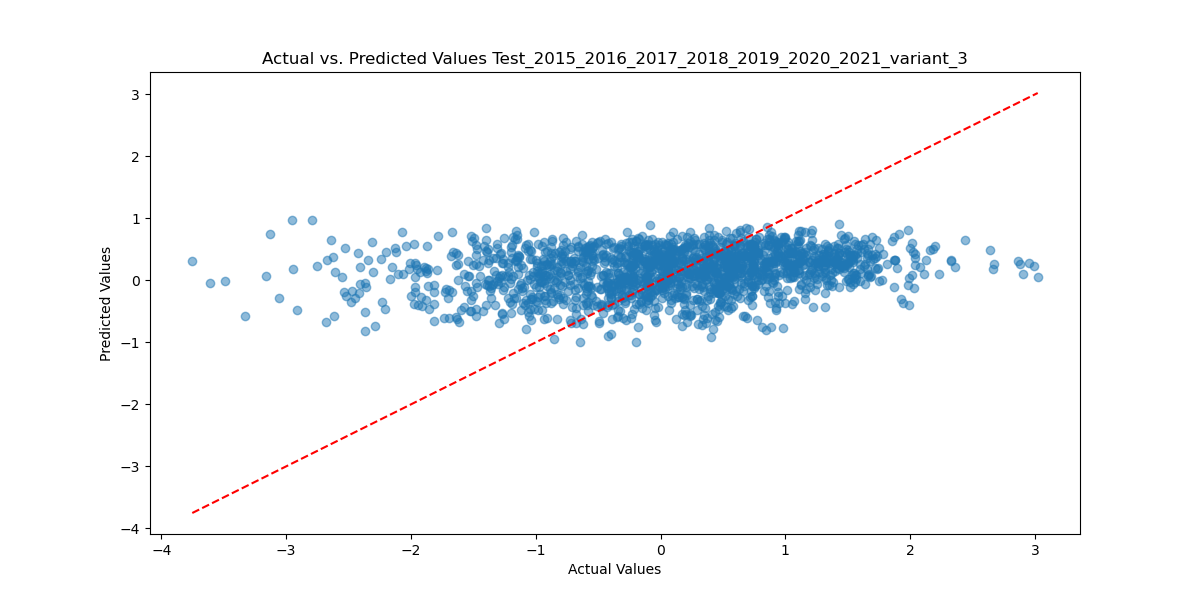
\includegraphics[width=1.0\textwidth]{./plots/scatter_Test_2015_2016_2017_2018_2019_2020_2021_variant_3.png}
	\caption{\label{fig:scatter_excluded_years_variant_3}This scatter plot shows the relationship between prediction and real values of excluded years (variant 3).}
\end{figure}
\subsubsection{Feature importance}
We get feature importance values for each Feature here the 10 most important features are shown (Table \ref{table:feature_importance_variant_3}).
As can be seen in the table the frost days in january are once again featured as most important followed by the SPI values. Even though it is questionable if it holds any meaning considering the bad performance of this model and the still relatively uniform distribution of feature importance values suggesting the model was not able to identify features with high predictive power.
\begin{table}[H]
	\centering
	\begin{tabular}{lc}
		\hline
		Feature                        & Importance \\
		\hline
		frost\_days\_monthly\_month\_1 & 0.067033   \\
		spi\_monthly\_month\_2         & 0.058844   \\
		spi\_monthly\_month\_1         & 0.057278   \\
		spi\_monthly\_month\_6         & 0.057119   \\
		spi\_monthly\_month\_3         & 0.055624   \\
		spi\_monthly\_month\_9         & 0.052494   \\
		spi\_monthly\_month\_4         & 0.051838   \\
		spi\_monthly\_month\_5         & 0.048565   \\
		spi\_monthly\_month\_8         & 0.046959   \\
		spi\_monthly\_month\_7         & 0.046922   \\
		\hline
	\end{tabular}
	\caption{\label{table:feature_importance_variant_3} Feature importance for variant three.}
\end{table}


\subsection{Variant 4}
This variant combines the raw climate data with the mean regional yield.
\subsubsection{Performance}
The model exhibits excellent performance on both the training and validation data with R2 scores of 0.97 and 0.82, respectively. While the R2 score decreases to 0.51 when all excluded years are considered, the model still performs relatively well on the excluded years.  The model shows good generalization ability, with R2 values ranging from 0.36 to 0.66 for individual excluded years.
This model performs the best among all tested variants. Showing that the raw climate data holds more predictive power compared to the choses derived features.
As can be seen in table \ref{table:errors_on_datasets_variant_4} and \ref{table:errors_on_datasets_years_variant_4}.
\begin{table}[H]
	\centering
	\begin{tabular}{lcccc}
		\hline
		Data Split                 & MSE  & RMSE & MAE  & R$^2$ \\
		\hline
		Training Data              & 0.02 & 0.15 & 0.12 & 0.97  \\
		Validation Data            & 0.17 & 0.41 & 0.31 & 0.82  \\
		Test (Excluded: 2015-2021) & 0.51 & 0.71 & 0.56 & 0.51  \\
		\hline
	\end{tabular}
	\caption{\label{table:errors_on_datasets_variant_4} Random Forest performance metrics for training, validation, and test sets. The test set excludes data from years 2015 to 2021 (variant 4).}
\end{table}

\begin{table}[H]
	\centering
	\begin{tabular}{lcccc}
		\hline
		Excluded Year & MSE  & RMSE & MAE  & R$^2$ \\
		\hline
		2015          & 0.35 & 0.59 & 0.45 & 0.65  \\
		2016          & 0.57 & 0.75 & 0.60 & 0.36  \\
		2017          & 0.38 & 0.62 & 0.49 & 0.56  \\
		2018          & 0.83 & 0.91 & 0.73 & 0.40  \\
		2019          & 0.45 & 0.67 & 0.52 & 0.66  \\
		2020          & 0.61 & 0.78 & 0.64 & 0.42  \\
		2021          & 0.36 & 0.60 & 0.48 & 0.52  \\
		\hline
	\end{tabular}
	\caption{\label{table:errors_on_datasets_years_variant_4} Random Forest performance metrics for test sets with individual years excluded.}
\end{table}

\begin{figure}[H]
	\centering
	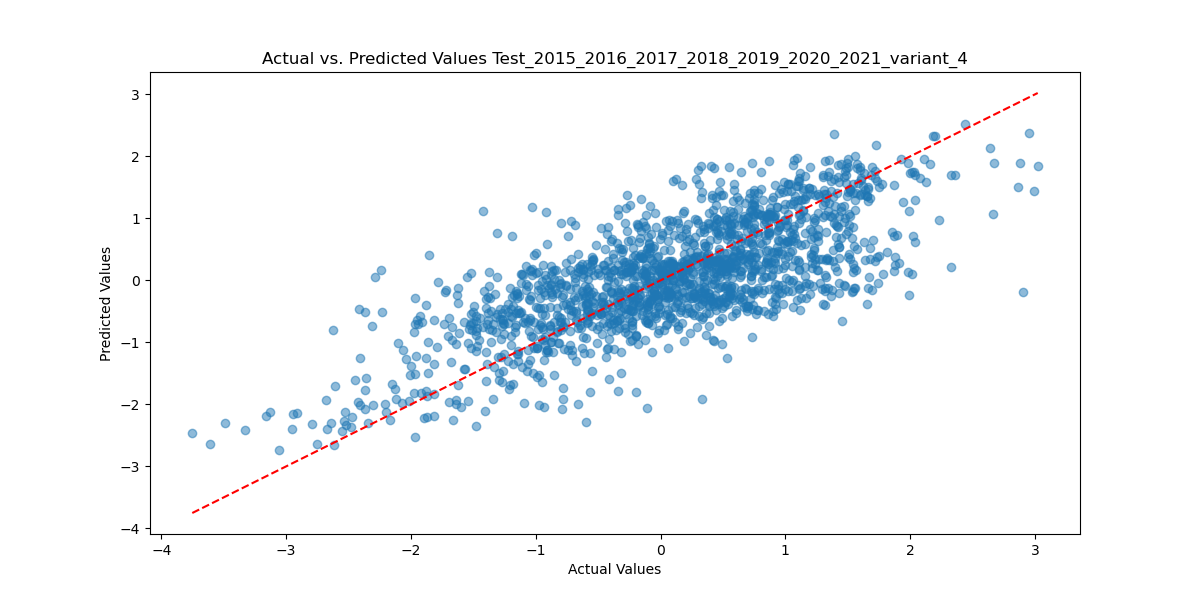
\includegraphics[width=1.0\textwidth]{./plots/scatter_Test_2015_2016_2017_2018_2019_2020_2021_variant_4.png}
	\caption{\label{fig:scatter_excluded_years_variant_4}This scatter plot shows the relationship between prediction and real values of excluded years (variant 4).}
\end{figure}

\subsubsection{Feature importance}
We get feature importance values for each Feature here the 10 most important features are shown (Table \ref{table:feature_importance_variant_4}).
Still the mean regional yield takes the top spot as the most important feature as expected. Followed by 8 of the 9 following top features being in may and june suggesting these month have a significant impact especially for humidity precipitation wind and solar radiation.
Temperature values are not featured in this top 10 list.
\begin{table}[H]
	\centering
	\begin{tabular}{lc}
		\hline
		Feature                    & Importance \\
		\hline
		mean\_regional\_ww\_yield  & 0.655228   \\
		hurs\_monthly\_month\_6    & 0.019800   \\
		pr\_monthly\_month\_5      & 0.017073   \\
		pr\_monthly\_month\_6      & 0.011238   \\
		sfcWind\_monthly\_month\_5 & 0.010490   \\
		rsds\_monthly\_month\_1    & 0.008350   \\
		rsds\_monthly\_month\_6    & 0.007603   \\
		sfcWind\_monthly\_month\_6 & 0.007448   \\
		hurs\_monthly\_month\_5    & 0.007200   \\
		rsds\_monthly\_month\_5    & 0.007129   \\
		\hline
	\end{tabular}
	\caption{\label{table:feature_importance_variant_4} Feature importance for variant four.}
\end{table}

\subsection{Variant 5}
This model only uses the raw climate data without the mean regional yield. Especially interesting compared to the variant 3 with the derived features.
\subsubsection{Performance}
The model shows good performance on the training data (R2: 0.95) and moderate performance on the validation data (R2: 0.59). However, when tested on the excluded years, the performance drops to R2 of 0.21 when all excluded years are considered.  Individual excluded years exhibit a wide range of R2 scores, from 0.08 to 0.34.  This suggests that the model is still capable of some generalization but could be improved further.
We can deduct that the raw climate data holds at least some predictive power for yield compared to the derived features but the performance is still not satisfactory when the mean regional yield is excluded
As can be seen in table \ref{table:errors_on_datasets_variant_5} and \ref{table:errors_on_datasets_years_variant_5}.
\begin{table}[H]
	\centering
	\begin{tabular}{lcccc}
		\hline
		Data Split                 & MSE  & RMSE & MAE  & R$^2$ \\
		\hline
		Training Data              & 0.05 & 0.22 & 0.17 & 0.95  \\
		Validation Data            & 0.39 & 0.62 & 0.48 & 0.59  \\
		Test (Excluded: 2015-2021) & 0.83 & 0.91 & 0.72 & 0.21  \\
		\hline
	\end{tabular}
	\caption{\label{table:errors_on_datasets_variant_5} Random Forest performance metrics for training, validation, and test sets. The test set excludes data from years 2015 to 2021 (variant 5).}
\end{table}

\begin{table}[H]
	\centering
	\begin{tabular}{lcccc}
		\hline
		Excluded Year & MSE  & RMSE & MAE  & R$^2$ \\
		\hline
		2015          & 0.67 & 0.82 & 0.67 & 0.34  \\
		2016          & 0.82 & 0.91 & 0.70 & 0.08  \\
		2017          & 0.75 & 0.87 & 0.68 & 0.13  \\
		2018          & 1.16 & 1.08 & 0.89 & 0.17  \\
		2019          & 0.90 & 0.95 & 0.77 & 0.32  \\
		2020          & 0.92 & 0.96 & 0.77 & 0.13  \\
		2021          & 0.56 & 0.75 & 0.57 & 0.27  \\
		\hline
	\end{tabular}
	\caption{\label{table:errors_on_datasets_years_variant_5} Random Forest performance metrics for test sets with individual years excluded.}
\end{table}

\begin{figure}[H]
	\centering
	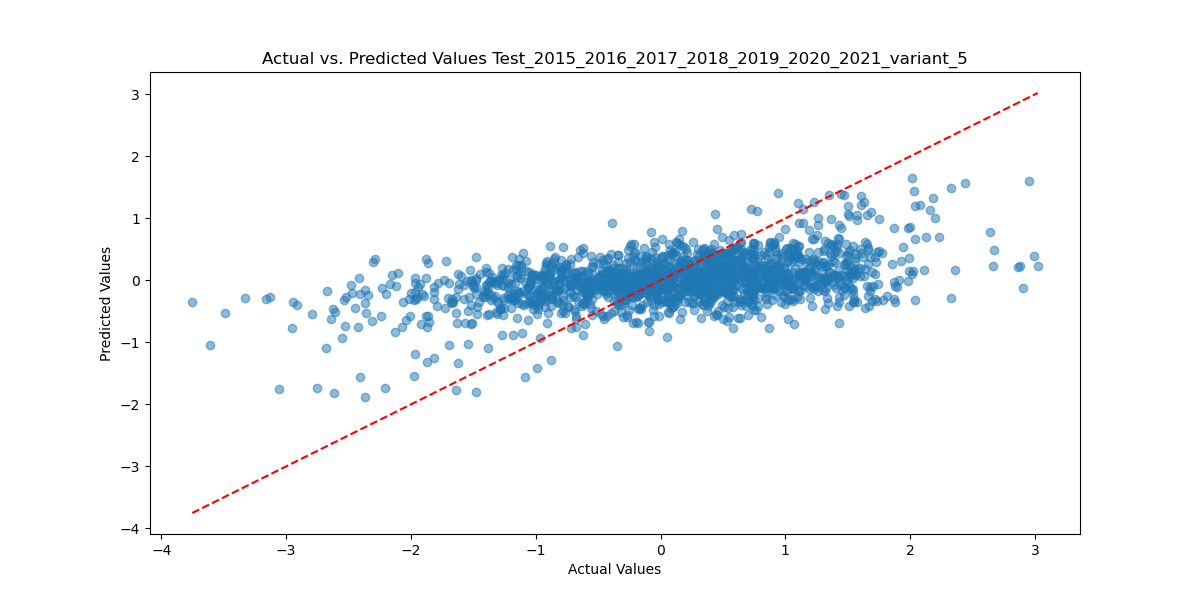
\includegraphics[width=1.0\textwidth]{./plots/scatter_Test_2015_2016_2017_2018_2019_2020_2021_variant_5.png}
	\caption{\label{fig:scatter_excluded_years_variant_5}This scatter plot shows the relationship between prediction and real values of excluded years (variant 5).}
\end{figure}

\subsubsection{Feature importance}
We get feature importance values for each Feature here the 10 most important features are shown (Table \ref{table:feature_importance_variant_5}).
\begin{table}[H]
	\centering
	\begin{tabular}{lc}
		\hline
		Feature                    & Importance \\
		\hline
		hurs\_monthly\_month\_6    & 0.044763   \\
		sfcWind\_monthly\_month\_5 & 0.034810   \\
		rsds\_monthly\_month\_8    & 0.031015   \\
		rsds\_monthly\_month\_1    & 0.030293   \\
		tasmin\_monthly\_month\_1  & 0.029628   \\
		pr\_monthly\_month\_5      & 0.028016   \\
		rsds\_monthly\_month\_2    & 0.026188   \\
		tasmin\_monthly\_month\_2  & 0.024988   \\
		pr\_monthly\_month\_4      & 0.023498   \\
		hurs\_monthly\_month\_5    & 0.022673   \\
		\hline
	\end{tabular}
	\caption{\label{table:feature_importance_variant_5} Feature importance for variant five.}
\end{table}


\section{Summary and Conclusions}
This experiment explored the use of random forest models to predict winter wheat yield anomalies in German NUTS3 regions. Five model variants were tested, each using different combinations of features, including mean regional yield, derived climate indices, and raw climate data. The results provide several insights:

\subsection{Model Performance}
\begin{itemize}
	\item Variant 4, which combined raw climate data with mean regional yield, performed best overall, achieving an R² of 0.51 on excluded test years.
	\item The inclusion of mean regional yield significantly improved model performance across variants, suggesting its importance as a predictor.
	\item Raw climate data (Variant 5) outperformed derived climate indices (Variant 3) when used without mean regional yield, indicating that the chosen derived features may not capture all relevant climate information.
\end{itemize}

\subsection{Feature Importance}
\begin{itemize}
	\item Mean regional yield consistently emerged as the most important feature when included.
	\item Climate variables in May and June appeared particularly influential, especially for humidity, precipitation, wind, and solar radiation.
	\item Surprisingly, temperature-related features were less prominent in the top-ranked features for the best-performing model (Variant 4).
\end{itemize}

\subsection{Limitations and Future Work}
\begin{itemize}
	\item The experiment's scope was limited, focusing on a single crop (winter wheat) and one machine learning algorithm (random forest).
	\item The model's performance on excluded years (2015-2021) was notably lower than on the validation set, suggesting potential overfitting or temporal dependencies not fully captured by the model.
	\item Feature engineering and selection could be improved, particularly for derived climate indices which showed limited predictive power.
	\item The random selection of validation data may not be ideal for time series data, potentially leading to information leakage.
	\item Hyperparameter optimization was limited to the number of trees, leaving room for further tuning.
\end{itemize}

\subsection{Future Directions}
To build upon this experiment, future work could:
\begin{itemize}
	\item Explore other machine learning algorithms, such as gradient boosting or neural networks.
	\item Implement more sophisticated time series cross-validation techniques.
	\item Investigate additional feature engineering approaches, potentially incorporating domain knowledge from agronomists.
	\item Extend the analysis to other crops and regions to test the model's generalizability.
	\item Incorporate additional data sources, such as soil quality or farming practices, to improve predictive power.
\end{itemize}

In conclusion, while this experiment demonstrates the potential of machine learning for crop yield prediction, it also highlights the complexities involved in modeling agricultural systems. The strong influence of historical regional yields suggests that local factors play a crucial role, emphasizing the need for models that can effectively combine climate data with region-specific characteristics. As climate change continues to impact agricultural systems, refining these predictive models will be crucial for ensuring food security and supporting adaptive farming practices.

\end{document}

